
\section{Map-Erkennung [H]}
Nachdem der Spieler der Lobby beigetreten ist, wird es Zeit für ihn die Spielumgebung zu zeichnen und diese für die
Abstimmung freizugeben. Das passiert, indem dieser einen QR-Code (``Quick Response''), welcher sich in der
Mitte der Lobby befindet, mit einem mobilen Endgerät, welches über eine Kamera verfügt, abscannt. Somit wird
er auf eine Webseite geleitet, welche wieder auf die Kamera zugreift. Auf dieser ist bereits eine Objekterkennung
vorprogrammiert. Auf die Funktionsweise und auf die technische Umsetzung wird im folgenden \dots eingegangen. Wenn der Spieler
merkt, dass die Objekterkennung das Blatt erkannt hat, kann dieser ein Bild aufnehmen. Im nächsten Schritt ist es nochmals möglich
die erkannten Kanten zu verschieben. Wenn sich der User für das Foto als Map entscheidet, so kann er den ausgewählten Teil in eine
top-down-2d-Perspektive
umwandeln. Kurzgesagt werden dabei die vier ausgewählten Ecken, welche über die Kanten des Blatt Papiers liegen,
für eine Perspektiven-Transformation
mit OpenCV2 herangezogen. Wenn der Spieler dann so weit ist, kann er dieses Bild beziehungsweise diese Map bestätigen und
sendet sie somit zurück an die Lobby. Dann kann die Abstimmung beginnen.

\begin{figure}[H]
    \centering
    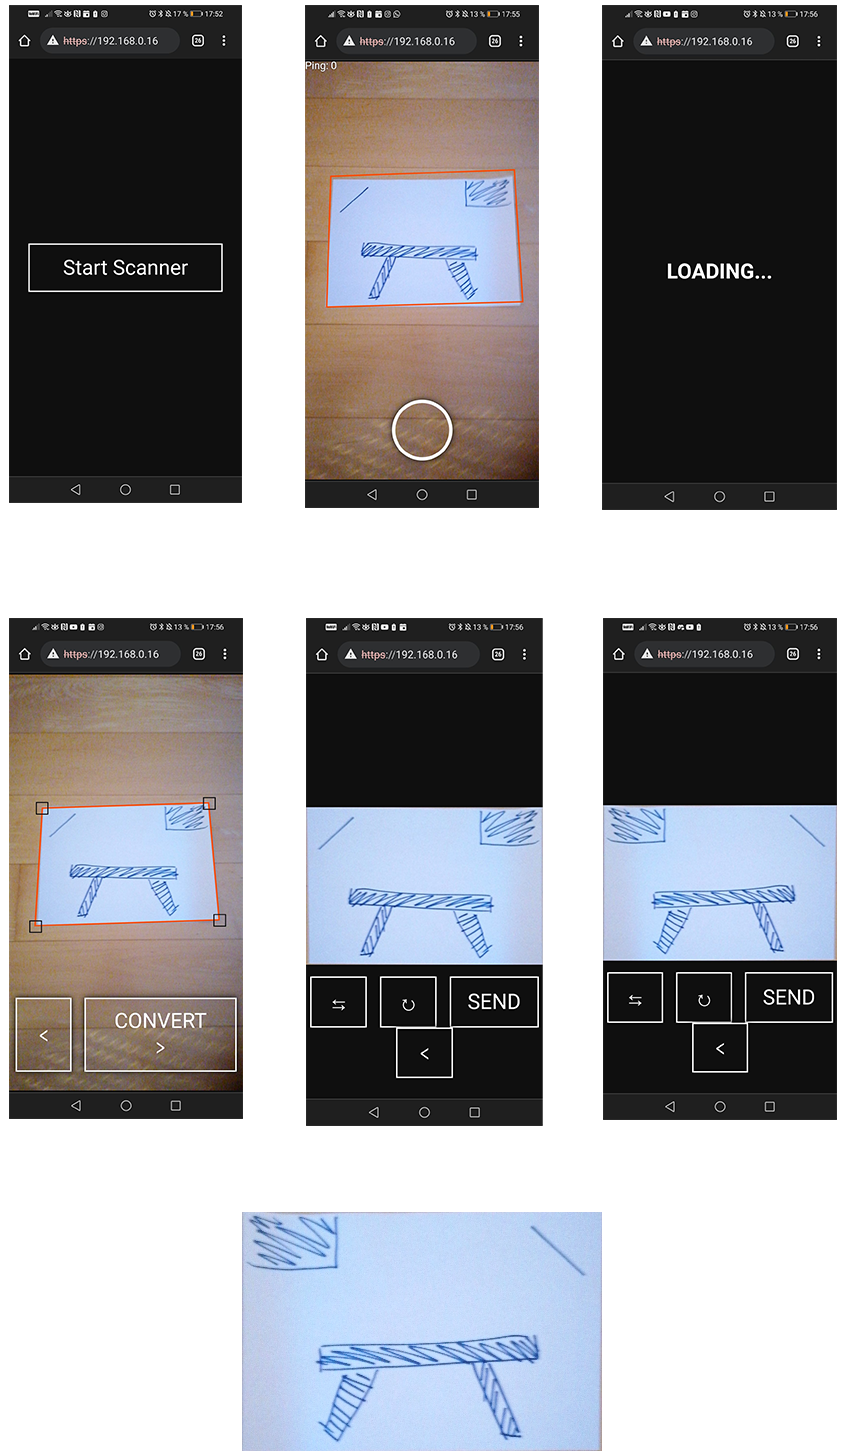
\includegraphics[scale=0.4]{pics/demo_maperkennung/sammlung_1.png}
    \caption{Screenshots der Maperkennungsanwenung}
    \label{fig:map:maperkennungsprozess}
\end{figure}

\setauthor{Himmetsberger Jonas}
\subsection{Objekterkennung [H]}
Das Thema ``Objekterkennung'' ist ein extrem schnell wachsendes und sich verbesserndes Feld in der Welt der Bildverarbeitung beziehungsweise
Bildanalyse. \\
Die Objekterkennung ist ein großer Teil der Arbeit. Hier wird aus dem live Footage der Kamera das Blatt Papier und anschließend
in einer fertigen Aufnahme die Map erkannt.
\\
\\
Die Objekterkennung wird zum Beispiel bei komplexen und großen Paketdiensten eingesetzt. Sollen Pakete nach Farbe gruppiert werden, so
reicht bereits ein Farbsensor. Das ist in den meisten Fällen jedoch nicht genügend.
Vielmals werden Pakete auf Strichcodes oder Adressen überprüft.
Wenn also unterschieden werden muss, wo welches Paket landen soll, so ist eine Kamera nötig. Diese muss
ein genügend gut auflösendes Bild aufnehmen, dass daraus Informationen gewonnen werden können. Diese Daten müssen zur Auswertung
mathematisch beschrieben werden. Zur Übersetzung werden Verfahren, wie Kantenerkennung, Transformationen oder Größen- und Farberkennung,
aber auch künstliche Intelligenzen
eingesetzt. In dieser Arbeit wurden Kanten zur Objekterkennung herangezogen.
Die Korrektheit des Ergebnisses ist abhängig von der Korrektheit der bereitgestellten Daten und wie genau das Objekt mathematisch
beschrieben werden kann.
\\
Ein weiteres Beispiel, wo Objekterkennung eingesetzt wird, ist in
Fahrerassistenzsysteme oder autonomes Fahren. Bereits in der ersten Stufe des autonomen Fahrens (dem assistierten Fahren)
werden zur Hilfe Kameras außerhalb des Fahrzeugs angebracht. In einem Auto, welches als Stufe eins autonomes Assistenzsystem
eingestuft wird, werden diese Kameras für einen automatischen Spurhalteassistenten eingesetzt. Via Bildanalyse und Objekterkennung
werden die Linien auf der Straße erkannt. \\
In höheren Stufen ist die Objekterkennung nicht mehr wegzudenken. Es müssen Verkehrsschilder und Personen auf der Straße erkannt
werden um daraufhin entsprechen zu agieren.

Andere Beispiele:
\begin{compactitem}
    \item Gesichtserkennung, um das Smartphone zu entsperren.
    \item Qualitätskontrolle, zur Erkennung und automatischen Entfernung von kaputten oder beschädigten Teilen.
    \item Personenerkennung, um Menschenmassen zu analysieren.
\end{compactitem}

\subsubsection{Beschreibung der Funktionalität [H]}

Wie schon erwähnt kann man aus Bildern Daten erkennen. Viele Pixel bilden insgesamt ein Bild, welches wir visuell aufnehmen und in welchem wir alles Mögliche erkennen können. Jeder einzelne dieser Pixel in einem digitalen Bild enthält Informationen über die Helligkeit und über die Farbe. Der Bildpunkt setzt sich zusammen aus den Farben Rot, Grün und Blau. Aus diesen drei können alle möglichen Farben abgebildet werden.
\\
Bevor ich darauf eingehe, wieso wir uns für die Konturenerkennung als Art der Bilderkennung entschieden haben, ist es noch entscheidend zu wissen, wie der Mensch Objekte erkennt.
\\
In unserem Auge passiert die Farberkennung via den Zapfen. Auch hier wird die Wellenlänge des Lichts in ein Gemisch aus Rot, Grün und Blau aufgeteilt. Allerdings benötigen wir das reine Farbsehen nicht um Objekte zu erkennen. Uns reicht es schon, wenn wir nur Informationen über die Helligkeit empfinden. Somit können wir zum Beispiel auch in Schwarz-Weiß-Bildern oder in der Dunkelheit bei wenig Licht Objekte erkennen. Wir erkennen einen Unterschied zwischen Objekten, welche sich in einem dreidimensionalen Raum befinden leicht, indem das eine Objekt sich in der Helligkeit von dem anderen Objekt unterscheidet. Das heißt, dass wenn z.B. ein Würfel auf einem Boden liegt, dann erkennen wir den Würfel, weil dieser anders viel Licht reflektiert als der Boden. Und an der Stelle, wo der Würfel aufhört, erkennen wir eine Kontur. Hier ist der Unterschied zwischen Boden und Würfel erkennbar.
\\
Und genau so passiert auch die Objekterkennung in unserem Spiel ScribbleFight. Hier wird zuerst aus der Live-View, welche vom Client zur Verfügung gestellt wird, das Farbbild in Graustufen konvertiert. Das passiert, indem für jeden Pixel ein ``Durchschnitts-Wert'' der Helligkeit von allen drei Farbwerte (Rot, Grün, Blau), welche in einem 8-Bit System von 0 bis 255 geht, gebildet wird. Wie dies jedoch genauer funktioniert, wird im Kapitel Bildverarbeitungsalgorithmen
\ref{maai:alogs}
genauer erklärt.

\begin{lstlisting}[caption=Alle unnötigen Bilddaten entfernen,language=Python,label=lst:impl:filters]
    def check(img):
        
        ...

        # CONVERT IMAGE TO GRAY SCALE
        imgGray = cv2.cvtColor(img, cv2.COLOR_BGR2GRAY)
        imgBlur = cv2.GaussianBlur(imgGray, (5, 5), 1)  # ADD GAUSSIAN BLUR
        upperThres = 40
        lowerThres = 40
        imgThreshold = cv2.Canny(
            imgBlur, upperThres, lowerThres)  # APPLY CANNY BLUR
        
        ...
\end{lstlisting}


Nachdem das Bild in ein Schwarz-Weiß-Bild umgewandelt wurde, muss vor der Konturenerkennung noch ein Schwellwert-Bild eines unscharfen Bildes erzeugt werden. In der Untenstehenden Abbildung \ref{fig:map:documentscanner}
das dritte Bild von links, oben. Das Schwellwert-Bild dient dazu, maximal viel Information aus dem Bild zu entfernen. Somit bleiben nur die relevanten Informationen über, welche OpenCV2 braucht um Konturen bilden zu können.

\begin{lstlisting}[caption=Erhalten von Konturen,language=Python,label=lst:impl:getContours]
        ...
        
        contours, hierarchy = cv2.findContours(
            imgThreshold, cv2.RETR_LIST, cv2.CHAIN_APPROX_SIMPLE)  # FIND ALL CONTOURS

        # FIND THE BIGGEST COUNTOUR
        accuracy = 25/1000
        area = 1000
        biggest, maxArea = biggestContour(
            contours, accuracy, area)  # FIND THE BIGGEST CONTOUR
        
        ...

        edges = getEdges(oldBiggest, biggest, contours, img, biggestChanged)

    return edges
\end{lstlisting}

In diesem Code-Block sieht man jetzt wie wir in unserer Diplomarbeit mit OpenCV2 die Konturen aus einem Schwellwert-Bild extrahiert haben und danach die größte Kontur herausgefunden haben. Wie die Funktion ``biggestContour(\dots)'' funktioniert ist in diesem Codeblock \ref{lst:impl:findBiggestContour} beschrieben. Und danach wird in ``getEdges(\dots)'' ein Numpy-Array von den Eckpunkten erzeugt, in eine anderer Reihenfolge, welche für den Perspektiven Transform relevant ist, umgewandelt und dann als Return-Wert zurückgegeben.

\begin{figure}[H]
    \centering
    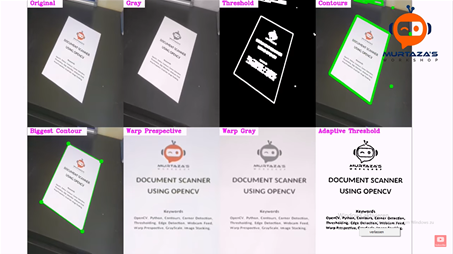
\includegraphics[scale=1]{pics/maperkennung/documentscanner.png}
    \caption{Documenten Scanner}
    \label{fig:map:documentscanner}
\end{figure}

Aus diesen Konturen, welche OpenCV2 erkennt, wird die größte, geschlossene Umrandung herausgesucht. Es wird davon ausgegangen, dass sich hier das fokussierte Objekt, also das Blatt Papier, befindet. Um nun die vier Eckpunkte lokalisieren zu können, wird eine vorgefertigte Funktion namens ``approxPolyDP'' angewendet. Diese legt, mit den übergebenen Parametern ein Viereck über die Konturen. Danach werden aus diesem Viereck die 4 Eckpunkte extrahiert und als Array wieder an den Client zurückgesendet.


\begin{lstlisting}[caption=approxPolyDP,language=Python,label=lst:impl:findBiggestContour]
    def biggestContour(contours, accuracy, areaVal):  # FIND THE BIGGEST CONTOUR
        biggest = np.array([])
        max_area = 0

        for i in contours:
            area = cv2.contourArea(i)
            if area > areaVal:
                peri = cv2.arcLength(i, True)
                # findet die vier Eckpunkte heraus und gibt diese zurueck
                approx = cv2.approxPolyDP(i, accuracy * peri, True)
                if area > max_area and len(approx) == 4:  # IF == 4 THEN SQUARE
                    biggest = approx
                    max_area = area
        return biggest, max_area
\end{lstlisting}

In der folgenden Funktion namens ``getWrappedImg(\dots)'', wird das Bild, welches aufgenommen wurde in eine zwei-dimensionale top-down Ansicht umgewandelt. Allerdings geschieht dies nur da, wo zuerst die Eckpunkte beziehungsweise das Blatt Papier (also die Spielumgebung) gefunden wurden. Wie dies funktioniert ist im folgenden Codeblock
\ref{lst:impl:convertPoints} ersichtlich.


Zuerst wird aus dem übergebenen ``snipset''-Parameter, welcher als Array vorliegt, die Daten ausgelesen und auf die Variablen ``pt\_A'' bis ``pt\_D'' geschrieben. Diese vier Buchstaben geben die Eckpunkte an. Aus diesen Eckpunkten wird im Folgenden dann ein Vektor erzeugt. Für weitere Berechnungen wird dann noch die länge zwischen den wahrscheinlich parallel zueinanderliegenden Vektoren AD und BC berechnet. Dies ist wichtig, um im späteren Code herauszufinden, in welcher Orientierung das Blatt Papier zu der Kamera liegt.

\begin{lstlisting}[caption=Bild in Vogelperspektive umwandeln,language=Python,label=lst:impl:convertPoints]
def getWrappedImg(img, snipset):
    snipset = squarify(snipset)

    pt_A = snipset[0]
    pt_B = snipset[1]
    pt_C = snipset[2]
    pt_D = snipset[3]

    lineAB = np.array([pt_A, pt_B])
    lineBC = np.array([pt_B, pt_C])
    lineCD = np.array([pt_C, pt_D])
    lineDA = np.array([pt_D, pt_A])

    width_AD = np.sqrt(((pt_A[0] - pt_D[0]) ** 2) + ((pt_A[1] - pt_D[1]) ** 2))
    width_BC = np.sqrt(((pt_B[0] - pt_C[0]) ** 2) + ((pt_B[1] - pt_C[1]) ** 2))
\end{lstlisting}
Im folgenden Code-Block passiert zuerst im Grunde genommen genau dasselbe, wie im zuvor erklärtem Code-Block \ref{lst:impl:convertPoints}. Hier wird die größere Länge der beiden Vektoren AB und CD, welche wahrscheinlich in der Realität parallel zueinander liegen, errechnet. Dabei wird angenommen, dass diese beiden Längen die Höhe des Blatt Papiers sind.
\begin{lstlisting}[language=Python,label=lst:impl:findBiggestLine,firstnumber=16]
    maxHeight = max(int(width_AD), int(width_BC))
    if maxHeight == width_AD:
        lineA = lineDA
    else:
        lineA = lineBC

    height_AB = np.sqrt(((pt_A[0] - pt_B[0]) ** 2) +
                        ((pt_A[1] - pt_B[1]) ** 2))
    height_CD = np.sqrt(((pt_C[0] - pt_D[0]) ** 2) +
                        ((pt_C[1] - pt_D[1]) ** 2))
    maxWidth = max(int(height_AB), int(height_CD))
    if maxWidth == height_AB:
        lineB = lineAB
    else:
        lineB = lineCD
\end{lstlisting}

Die nun errechnete maximale Höhe wird nun noch mit einem realistischen Faktor multipliziert, um noch ein akkurateres Ergebnis der Perspektiventransformation erzielen zu können. Dieser ``realistische Faktor'' wird errechnet, indem der Winkel zwischen den beiden größten orthogonal zueinander liegenden Linien in folgende Formel miteinbezogen wird:
\[ factor
    = \dfrac{90}{(180-angle)}
\]
Dieser errechnete Faktor staucht die Höhe eines Bildes, welches von der unteren Blattkante aufgenommen wurde und streckt die Höhe von jene, welche, wieso auch immer, von oben Blattkante aufgenommen wurden.


\begin{lstlisting}[language=Python,label=lst:impl:angle,firstnumber=31]
    angle = ang(lineA, lineB)
    if angle == 90:
        factor = 1
    if angle > 90:
        factor = 90 / (180-angle)
    if angle < 90:
        factor = 90 / angle

    maxHeight *= factor
\end{lstlisting}

Im letzten Teil der Funktion wird lediglich nur noch das Bild in die richtige Perspektive transformiert. Dies wird erzielt, indem man die beiden vorgefertigten Funktionen ``cv2.getPerspectiveTransform(\dots)'' und ``cv2.warpPerspective(\dots)'' verwendet. Als Return-Wert liefert die genannte Funktion ein Bild mit dem Datentypen OpenCV2, welches dann im späteren Verlauf noch umcodiert werden muss.

\begin{lstlisting}[language=Python,label=lst:impl:wrapPerspective,firstnumber=40]
    m = np.array([pt_A, pt_B, pt_C, pt_D])
    m = rotateCW(m)
    input_pts = np.float32(m)
    output_pts = np.float32([[0, 0],
                            [0, maxHeight - 1],
                            [maxWidth - 1, maxHeight - 1],
                            [maxWidth - 1, 0]])

    M = cv2.getPerspectiveTransform(input_pts, output_pts)

    dst = cv2.warpPerspective(
        img, M, (int(maxWidth), int(maxHeight)), flags=cv2.INTER_LINEAR)

    return dst
\end{lstlisting}


\subsection{Open-CV2 [H]}
\subsubsection{Bildverarbeitungsalgorithmen} \label{maai:alogs}
\dots
\subsubsection{Grayscale}\label{maai:grayscale}
\dots
\subsubsection{Blur}
\dots
\subsubsection{Thresholding}
\dots
\subsubsection{Detecting Contours}
\dots
\subsubsection{ApproxPolyDP}
\dots
\subsubsection{Wrap Perspective}
\dots

\subsubsection{Umwandlung der Bilder in für das Spiel brauchbare Daten [H]}
Hat man nun das Bild Perspektiven transformiert, so kann man dies mit dem Send-Button (Wie in Abbildung \ref{fig:map:maperkennungsprozess} ersichtlich) bestätigen.
Somit wird das Bild an den Python-Server ein letztes Mal zurückgesendet und es wird eine spielbare Map daraus generiert.
Wie dies Funktioniert wird in den folgenden Codeblöcken ersichtlich.

Zuerst wird sich wieder darum gekümmert, dass die Daten so stark minimiert werden, dass sie trotzdem noch brauchbar sind, aber so viel wie möglich Informationen beinhalten. Das heißt: so wenig wie möglich Bildmaterial soll so viel wie möglich Information enthalten. Doch davor wird das übergebene Bild in den RGBA-Farbraum umgewandelt und in ein OpenCV2-Bild konvertiert. Im RGBA Farbraum ist es zusätzlich noch möglich neben den Farbwerten auch Informationen über die Transparenz des Bildes abzuspeichern. Dann startet wieder dasselbe Prozedere, wie bei der Perspektiven Transformation.

Zuerst wird das Bild in Graustufen konvertiert. Wie dies funktioniert ist bereits im Unterpunkt \ref{maai:grayscale} erklärt. Dann wird es unscharf gezeichnet und danach ein adaptiver Threshold (ein Schwellwert-Bild) daraus generiert.

Im nächsten Schritt wird die vorgefertigte Funktion ``Bitwise\_not'' angewendet. Hier wird das Bild in nur schwarze und weiße Pixel umgewandelt. Sie wandelt also alle Pixel entweder in schwarze oder weiße Bildpunkte um und generiert daraus wieder ein neues OpenCV2 Bild. Auch dieses Bild wird wieder unscharf gezeichnet.

Was dann noch für das Spiel wichtig ist, ist, dass das Bild in einen Quader umgewandelt wird. Das heißt, dass das Schwellwert-Bild so umgewandelt wird, dass alle Seiten (Höhe und Breite) gleich lang sind. Die leeren Flächen, die daraus entstehen werden mit transparenten Pixeln gefüllt.

Die Zeile zwanzig dient dazu das Bild testweise in einem Ordner abzuspeichern.

\begin{lstlisting}[language=Python,caption=Bild in Spielbare Map umwandeln,label=lst:umsetzung:getplayablearray]
    def getPlayableArray(img):
        np.set_printoptions(threshold=sys.maxsize)

        alpha_img = cv2.cvtColor(img, cv2.COLOR_BGR2BGRA)  # rgba
        imgWarpGray = cv2.cvtColor(alpha_img, cv2.COLOR_BGR2GRAY)
        blurred = cv2.GaussianBlur(imgWarpGray, (7, 7), 0)
        imgAdaptiveThre = cv2.adaptiveThreshold(
            blurred, 255, cv2.ADAPTIVE_THRESH_GAUSSIAN_C, cv2.THRESH_BINARY_INV, 7, 2)
        imgAdaptiveThre = cv2.bitwise_not(imgAdaptiveThre)
        imgAdaptiveThre = cv2.medianBlur(imgAdaptiveThre, 3)

        # make image square
        imgAdaptiveThre = np.array(makeSquare(
            cv2.cvtColor(imgAdaptiveThre, cv2.COLOR_BGR2BGRA)))

        img = cv2.cvtColor(imgAdaptiveThre, cv2.COLOR_BGR2BGRA)

        # pippoRGBA2 = Image.fromarray(np.array(img).astype('uint8'), mode='RGBA')
        # pippoRGBA2.show()
        cv2.imwrite('./source/prototypes/streamFusion/output/imgAdaptiveThre.png', imgAdaptiveThre)
\end{lstlisting}

Im nächsten Schritt wird der Array berechnet, welcher als Grundlage für die spielbare Map dient und aus dem aufgenommenen Bild extrahiert wird. Der Array beinhaltet nach der Verarbeitung schwarze und transparente Bildpunkte. Die schwarzen Pixel symbolisieren jene Plätze, auf welchen sich der Spieler schlussendlich bewegen kann. Die transparenten Pixel sind jene, welche als Hintergrund erkannt wurden und somit nicht für den Spieler begehbar sein sollten. Wie sich jedoch der Spieler auf diesen Punkten bewegen kann und wie der Array in die Spiellogik implementiert wird, wird im Kapitel ``Erstellung der Spielumgebung \ref {impl:Spielumgebung}‘‘ von Rafetseder Tobias näher erklärt.

Jedoch wird zuerst eben das transformierte Bild in den Array umgewandelt. Dafür wird aus diesem adaptiven Threshold-Bild (Schwellwert-Bild) ein Faktor ausgerechnet, mit welchem die Bildpunkte zusammengefasst werden müssen, um insgesamt nicht mehr als \(\approx\)3025 Pixel zu überschreiten. Die dabei verwendete Formel wird im Folgenden an einem einfachen Beispiel erklärt. Diese lautet:

\[
    n \approx math.ceil(\sqrt{ \frac{ rows * columns }{ meshes } })
\]

Setzt man nun eine Bildbreite und eine Bildhöhe in ``rows'' und ``columns'' ein, so erhält man den ganzzahligen Faktor, mit welchem die angegebene Bildbreite und Höhe multipliziert werden muss, um maximal \(\approx\)3025 Pixel zu erreichen.
Angenommen also, das Bild ist 1920x1080 Pixel groß, so würde das eine Anzahl von 2.073.600 Pixel liefer. Setzt man diese Werte nun in die Formel ein, so erhält man den Faktor 27. Dividiert man nun die beiden Bildmaße mit diesem Wert, so erhält man ein Bild, welches 72x40 groß ist und somit eine Anzahl von 2880 Pixel liefert und somit weit unter den geforderten 3025 Pixeln liegt.

Der Grund, warum der Array eine maximale Größe von 3025 Einträgen hat, ist, weil p5.js, die Bibliothek, welche wir verwenden, um die Spielumgebung aufzubauen nur ein Maximum von 1000 Meshes generieren kann, bevor das Spiel zu ruckeln beginnt. Und wir gehen davon aus, dass man nie mehr als ein Drittel seines Blattes vollzeichnen wird.

Dann wird in einer zweidimensionalen Schleife das Bild durchgegangen und jeweils alle n Pixel ein Mittelwert errechnen über die Farbwerte des Bildes errechnet und somit der Hintergrund vom Vordergrund getrennt. Alle n Pixel werden zusammengefasst. Wenn in diesem Code also mehr als 95\% der Pixel Hintergrund darstellen, so wird der Pixel auch als Hintergrund gewertet (es wird also in den Map-Array ein transparenter Pixel an der Stelle x/n und y/n gepusht). Ansonsten wird ein Schwarzer Pixel (als Map erkannt) dem Map-Array hinzugefügt. An dem Punkt mit den Koordinaten x/n und y/n befindet sich also der neue Bildpunkt, da das Bild ja komprimiert werden soll.

Dieser Map-Array wird dann in ein File abgespeichert. Dieses File dient rein dazu, um den Array debuggen zu können. Darunter wird ein Bild, welches aus diesem Map-Array generiert worden ist, im angegebenen Pfad gespeichert.

\begin{lstlisting}[language=Python,label=lst:umsetzung:getArray,firstnumber=21]
        iar = np.asarray(img).tolist()

        rows = len(iar)
        columns = len(iar[0])

        meshes = 3025
        # percent = perc(rows * columns)
        percent = 95
        n = math.ceil(np.sqrt(rows * columns / meshes))
        x = 0
        y = 0

        newImg = []

        while y < rows:
            newImg.append([])
            while x < columns:

                i = 0
                j = 0
                bg = 0
                while i < n:
                    while j < n:
                        if (y + j) < rows and (x + i) < columns:
                            if np.all(iar[y + j][x + i][:3] == [255, 255, 255], 0):
                                bg += 1
                        else:
                            bg += 1
                        j += 1
                    j = 0
                    i += 1

                bgPercent = bg / (n**2)
                if (bgPercent < (percent / 100)):
                    newImg[int(y / n)].append([0, 0, 0, 255])
                else:
                    newImg[int(y / n)].append([255, 255, 255, 0])

                x += n
            x = 0
            y += n

        iar = np.asarray(newImg).tolist()
        with open('./source/prototypes/streamFusion/output/mapArray.txt', 'w') as f:
            f.writelines(repr(iar))

        # pippoRGBA2 = Image.fromarray(np.array(newImg).astype('uint8'), mode='RGBA')
        # pippoRGBA2.show()
        cv2.imwrite(
            './source/prototypes/streamFusion/output/newImg.png', np.array(newImg))

        return newImg

\end{lstlisting}
\subsection{Kommunikation mit der Lobby via Flask und Flask SocketIO [W]}

\section{KI [H]}
Im Laufe der Ausarbeitung der Diplomarbeit und der damit zusammenhängenden Forschung änderte sich oft die
Vorstellung darüber, wie das Endprodukt (KI) auszusehen hat, beziehungsweise, wie dieses aussehen kann.
Limitierungen, welche vor der Forschung noch nicht bekannt und bewusst waren, begrenzten die Lernfähigkeit der KI.
Auf Probleme, Lösungen und Ergebnisse wird jedoch noch näher in ... eingegangen.
\subsection{Lernen mit OpenAI-Gym [H]}
% \subsection{Künstliche Intelligenz Definition [H]}
\subsection{Reinforcement Learning [H]}
\subsection{Die ScribbleFight-KI [H]}
\subsubsection{Beschreibung der Funktionalität [H]}
\subsubsection{Warum Python? [H]}
\subsection{Tensorflow und Keras [H]}
\subsubsection{Tensorflow [H]}
\subsubsection{Keras [H]}
